\documentclass[../../norme-di-progetto.tex]{subfiles}

\begin{document}

\subsubsection{Finalità}%
\label{subs:accertamento_della_qualita/finalita}

GruppOne istanzia il processo di accertamento della qualità per garantire qualità di processo e di prodotto.
Gli esiti dei processi di verifica e validazione saranno indispensabili nello svolgimento del processo di accertamento della qualità.

\subsubsection{Descrizione}%
\label{subs:accertamento_della_qualita/descrizione}

Il processo di accertamento della qualità garantisce che i prodotti e i processi del ciclo di vita del software rispettino i requisiti prestabiliti e che aderiscano ai piani esecutivi prefissati.
Gli obiettivi e le strategie che il team si impegna ad applicare durante lo svolgimento del progetto sono presentati nel \textit{Piano di qualifica (versione \versione)}.

\subsubsection{Attività}%
\label{subs:accertamento_della_qualita/attivita}

Le principali attività coinvolte nel processo di accertamento della qualità sono:

\begin{description}
  \item [Pianificazione] si cercano le metodologie, le procedure, gli strumenti e le attività offerte da altri processi di supporto per organizzare le pianificazione della qualità.
  \item [Implementazione] si utilizza ciò che si è individuato al punto precedente per effettuare controlli di qualità sui processi e sui prodotti in atto.
  \item [Documentazione dei risultati] i risultati dei controlli di qualità dovrebbero essere poi documentati.
\end{description}

\paragraph{Denominazione delle metriche}%
\label{par:denominazione_delle_metriche}

Le metriche sono essenziali per avere una misura oggettiva di qualità del nostro prodotto, e vengono definite durante la pianificazione del processo di accertamento della qualità.
Per tale ragione per la definizione delle metriche di qualità è necessario identificare una denominazione comune.
Ogni metrica avrà la seguente struttura:
\begin{center}
  \textbf{M[Tipo][Sigla]}
\end{center}
\begin{description}
  \item [Tipo] indica il tipo di metrica. Può essere:
        \begin{itemize}
          \item PS -metrica di processo.
          \item PR -metrica di prodotto.
        \end{itemize}
  \item [Sigla] indica una sigla che abbrevia la metrica.
\end{description}

\paragraph{Accertamento qualità di prodotto}%
\label{par:accertamento_qualita_di_prodotto}
L'attività di accertamento della qualità di prodotto assicura la qualità dei prodotti realizzati e promuove controlli continui che possano prevenire danni irreparabili al termine del progetto.
È fortemente dipendente dalla qualità di processo: da processi privi di qualità, infatti, non è possibile ottenere buoni prodotti.

\subparagraph{Standard di riferimento}%
\label{subp:accertamento_qualita_di_prodotto/standard_di_riferimento}

Il riferimento principale che adottiamo per questo asse di qualità è lo standard ISO/IEC 25010:2011, ponendo particolare attenzione alle caratteristiche che hanno maggiore interesse per il proponente del prodotto.

\paragraph{Accertamento qualità di processo}%
\label{par:accertamento_qualita_di_processo}
L'attività di accertamento della qualità di processo monitora i processi istanziati. Per avere un sistema di accertamento della qualità di processo che funzioni è necessario che:

\begin{itemize}
  \item Si individuino i processi da controllare.
  \item Si stabiliscano le metriche di valutazione del processo.
  \item Si eseguano accertamenti continui sui processi scelti.
  \item In base ai risultati ottenuti, si ricerchi un miglioramento dei processi.
\end{itemize}

\subparagraph{Standard di riferimento}%
\label{subp:accertamento_qualita_di_processo/standard_di_riferimento}

Per questo asse di qualità lo standard principale che adottiamo è ISO/IEC 90003:2014, our considerando che per la natura del progetto la sua applicazione avrà portata limitata allo svolgimento del progetto stesso.

\subparagraph{PDCA}%
\label{subp:PDCA}
Il ciclo di Deming o ciclo PDCA è un processo iterativo per il monitoraggio e il miglioramento dei processi. Sfrutta la ripetizione di quattro attività:

\begin{description}
  \item [Plan] definisce gli obiettivi, le attività e i processi necessari per raggiungere i risultati attesi.
  \item [Do] esegue ciò che è stato definito nella fase di pianificazione.
  \item [Check] verifica gli esiti dei processi.
  \item [Act] esegue azioni correttive per migliorare la qualità dei processi.
\end{description}
\begin{figure}[H]
  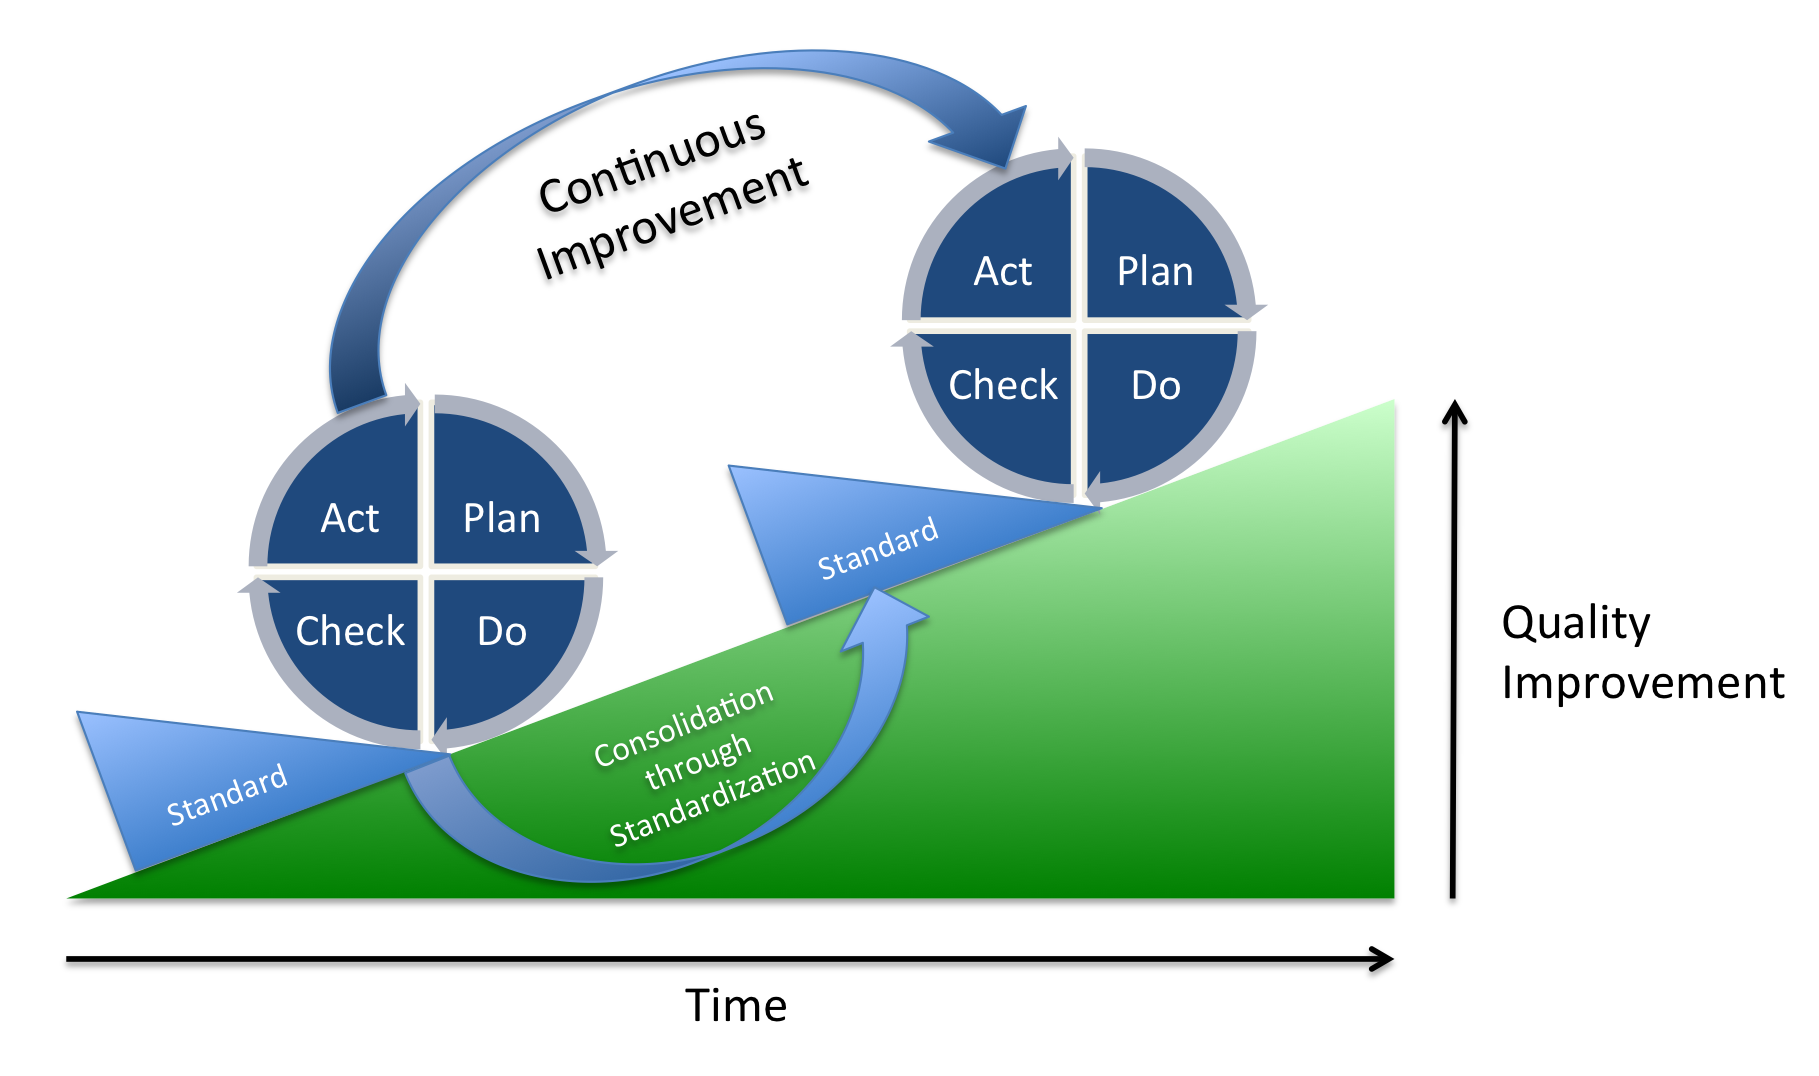
\includegraphics[width=8cm]{PDCA-process.png}
  \centering
  \caption{ciclo di Deming o PDCA.}
\end{figure}

\end{document}
